\chapter{Empirical evaluation of compression algorithms}
In this chapter, we compare lossless and lossy algorithms in terms of compression performance using both real and 
generated time series data. The lossless compression algorithms that we have chosen are Gorilla, LZ4,
Deflate and Zstandard. For the lossy algorithm part, we take a look at how PCM and PLA perform against each other.

\section{Datasets}
For these benchmarks, we have used three different datasets. The first dataset was generated from the
Time Series Benchmark Suite, a project mantained by TimescaleDB \cite{timescale_2019_timescaletsbs}.
The second dataset was provided by Dynatrace. Dynatrace is a Software Intelligence platform with a strong
emphasis on application performance monitoring. The datasets consist of metrics gathered from
different hosts running a wide range of applications under different loads.
The third dataset was provided by the New York Taxi and Limousine Commisson (TLC), and it constists
of records representing taxi trips, including information such as duration of the trip, amount
charged, tip amount \cite{tlc2019_dataset}.

\section{Methodology}
For the lossless algorithms, we have chosen to evaluate Gorilla performance against general-purpose
algorithms with generated and real-time series data. The metric in which we are interested is the
compression ratio, while we don't evaluate compression speed as this is dependent of the implementations we have
chosen. We have created a Java program that reads data from the input stream and returns the compression ratio
achieved by the algorithm selected. We decided to use Java because we could easily find implementations for
all the algorithms listed above. The program requires to specify the format of the dataset provided and the
algorithm to use for compression, as the following listing illustrates.
\lstset{
    basicstyle=\small,
    stringstyle=\ttfamily
}
\begin{lstlisting}[language=bash]
  $ ./gradlew shadowJar
  $ java -jar
  TimeseriesCompressionBenchmarks-all.jar [format] [algorithm]
\end{lstlisting}
The code is available on github \cite{dovidio_2019_dovidiotscompressionthesis}.
For gorilla compression, we have used an open source java implementation of the algorithm
\cite{burmanm_2018_burmanmgorillatsc}. Deflate, on the other hand, is already present in the the package
\textit{java.util.zip}, using the zlib library under the hood \cite{a2019_deflater}.
For LZ4 and ZStandard we have used open source implementations \cite{lz4_2019_lz4lz4java}\cite{luben_2015_lubenzstdjni}.
For creating/collecting time series data we have used NodeJs scripts, while data analysis and preprocessing
was done in python using numpy and pandas libraries.

\subsection{Generating devops data}
As we have mentioned before, we have used the TimeSeries Benchmark Suite to generate fake devops data.
This utility allows to specify which use case to simulate data for, which time interval between each data points
to use, the starting timestamp and the ending timestamp, how many hosts to simulate.
We have decided to generate data points every minute, for a single host and for 5 different time intervals:
2 hours, 4 hours, 8 hours, 16 hours and 48 hours. For each of this intervals we generate 50 different time series.

\subsection{Collecting Dynatrace Data}
Dynatrace provides a REST Api to retrieve metrics of entities monitored by it \cite{a2013_metrics}.
We have used this Api to retrieve data of several hosts which were monitored in one of the demo environment
Dynatrace uses for testing purposes.
The metrics we have chosen to collect are the following:
\begin{itemize}
    \item Host CPU Usage: Percentage of overall CPU usage
    \item Host CPU System: Percentage of CPU time used by the kernel
    \item Host CPU User: Percentage of CPU time used by user space processes
    \item Host CPU Io Wait: Percentage of CPU time spent waiting for input/output operations
    \item Host Memory Used: Percentage of memory used
    \item Host Memory Usage: Memory usage in bytes
    \item Host Disk Read Time: Disk read time in milliseconds
    \item Host Disk Write Time: Disk write time in milliseconds
\end{itemize}

\subsection{Taxi Data}
This dataset was provided by the New York Taxi and Limousine Commisson. For each month of the year
the TLC provide a data set for the two different taxi companies running in New York (green and yellow)
and for limousines. We have decided to take into account only yellow taxi data for one month.
Moreover, to make in memory compression feasible, we have dropped the last 3 millions records from the
dataset. Additionally, all the columns containing string data were removed since they are not handled
by the Gorilla algorithm.

\section{Results}
\subsection{Generated data}
Figure~\ref{devops_lossless_compression} illustrates the result of applying different compression algorithms
with generated data. It clearly shows how Gorilla is outperforming the other lossless comtrapression algorithms.
It is also interesting to notice how ZStandard and Deflate performs in a similar way, while LZ4 has
consistently the worst compression ratio, as one might have predicted from the literature.

\begin{figure}[!htbp]
\begin{center}
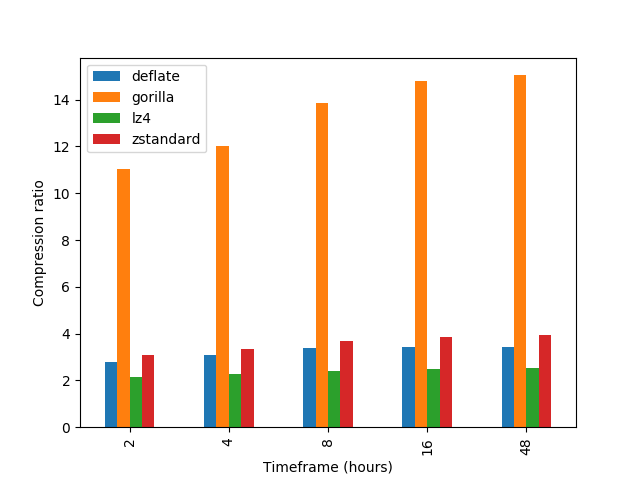
\includegraphics[width=300pt]{devops_bar_chart}
\caption[compression]{Generated data compressed with Gorilla, Deflate, ZStandard, LZ4.
Higher values indicates higher compression ratios.}
\label{devops_lossless_compression}
\end{center}
\end{figure}

\subsection{Dynatrace Data}
Results of the different compression algorithms applied to real-word series data are shown in
Figure~\ref{dynatrace_compression}. The results are similar to what we have seen for generated data,
with Gorilla outperforming general purposes algorithm across all metrics.

\begin{figure}[!htbp]
\begin{center}
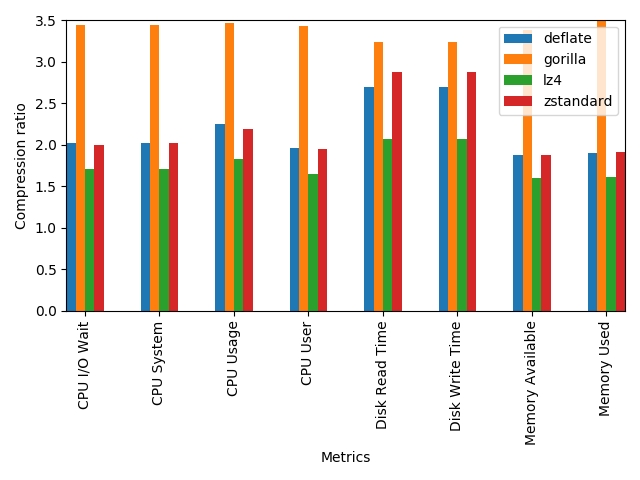
\includegraphics[width=300pt]{dynatrace_bar_chart}
\caption[compression]{Real world data collected by Dynatrace compressed with Gorilla, Deflate, ZStandard, LZ4.
Higher values indicates higher compression ratios.}
\label{dynatrace_compression}
\end{center}
\end{figure}

\subsection{Taxi Data}
For taxi data, we have decided to transform the data in a column format.
Since each record contains 15 columns, this means that we have transormed data in 15 time series,
ordered by pick up time.
Each time series data point represent a specific value for a specific taxi trip.
The time interval between each data point is not regular as in the previous data sets, for this
reason Gorilla delta of delta timestamp compression is likely to not yield good compression
ratios.
As Figure~\ref{taxi_bar_chart} shows, Gorilla compression does not perform well for this use case.
Its performance is on par with LZ4, while both Deflate and ZStandard achieve better compression ratio.

\begin{figure}[!htbp]
\begin{center}
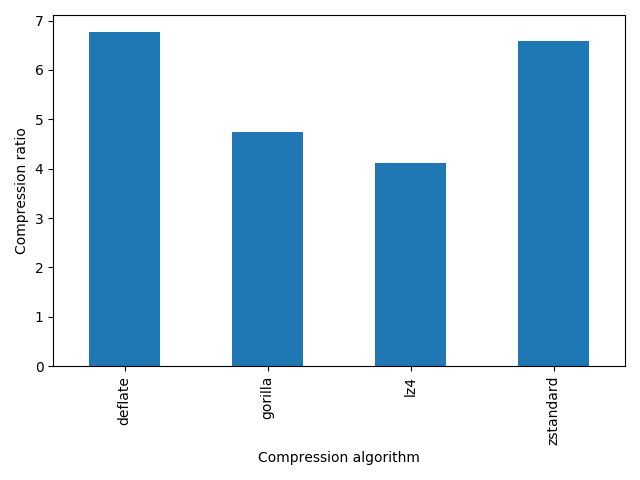
\includegraphics[width=300pt]{taxi_bar_chart}
\caption[compression]{Taxi Data compressed with Gorilla, Deflate, ZStandard, LZ4.
Higher values indicates higher compression ratios.}
\label{taxi_bar_chart}
\end{center}
\end{figure}